{
% Set the overall layout of the tree
\tikzstyle{level 1}=[level distance=2.5cm,sibling distance=3cm]
\tikzstyle{level 2}=[level distance=2.5cm,sibling distance=3cm]

% Define styles for bags and leafs
\tikzstyle{bag}=[rectangle,draw=black,text width=4em,text centered]
\tikzstyle{end}=[circle,draw=black,minimum width=3pt,fill,inner sep=0pt]

\begin{figure}
	\centering
	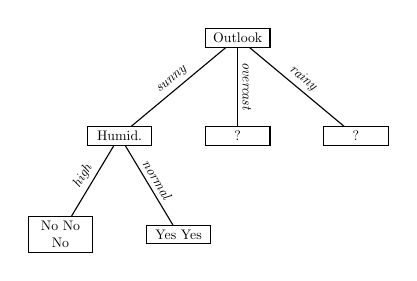
\begin{tikzpicture}[
		scale=0.5,
		every node/.style={scale=0.5},
		sloped
	]
		\node[bag]{\highlight{Outlook}}
    		child {
     	   		node[bag]{\highlight{Humid.}}
			child {
				node[bag,align=center]{No No\\No}
     	     		      	edge from parent
     		           	node[above]{\textit{high}}
			}
			child {
				node[bag,align=center]{Yes Yes}
                			edge from parent
                			node[above]{\textit{normal}}
			}
            		edge from parent 
            		node[above]{\textit{sunny}}
    		}
		child {
			node[bag]{?}
			edge from parent
			node[above]{\textit{overcast}}
		}
    		child {
        			node[bag]{?}
        			edge from parent         
            		node[above]{\textit{rainy}}
		};
	\end{tikzpicture}
\end{figure}}